\documentclass{article}
\usepackage{a4}
\usepackage{amsmath}
\usepackage{amsthm}
\usepackage{amssymb}
\usepackage{indentfirst}
\usepackage{verbatimbox,hyperref}
\usepackage[T1]{fontenc}
\usepackage[utf8]{inputenc}
\usepackage{tikz}
\usetikzlibrary{matrix}
\def\leftbracket{[}
\def\rightbracket{]}
\usepackage{tikz}
\usetikzlibrary{shapes,arrows,calc}
\newcommand{\data}{data \nodepart{second} \phantom{null}}
\usetikzlibrary{matrix,positioning,arrows.meta,arrows}

\tikzstyle{ptr}  = [draw, -latex']
\tikzstyle{head} = [rectangle, draw, text height=3mm, text width=3mm, text centered, node distance=3cm, inner sep=0pt]
\tikzstyle{data} = [rectangle split, rectangle split parts=2, draw, text centered, minimum height=3em]


\title{Graph Storage: How good is CSR really?}
\author{Mahammad Valiyev}

\begin{document}
\maketitle

\begin{abstract}
  In the last decade, the data size is growing exponentially and processing those data is becoming a difficult problem. Nowadays researchers and industry have been interested in the analysis of the graph to get deep understanding of social networks. Many of these graphs used in industry have become very large, containing hundreds of millions of nodes and edges. In this paper, I propose Compressed Sparse Row(CSR) which is a fast graph container. My CSR implementation also supports updates on graph. On a static graph, CSR gives ~1.2-3x better performance over Adjacency List Implementation(AL) on Depth-First-Search(DFS) and Breadth-First-Search(BFS) and up to 2-3x better performance on Dijkstra algorithm(Shortest path).
\end{abstract}
\textbf{Keywords:} Graph databases, Compressed Sparse Row

\section{Introduction}
Graph analysis have become more popular in the last few years. Graphs are usually used to represent social networks in which vertices indicate users and edges indicate friendship between users. Facebook has 1.39 billion  active users as of 12/2014 with more than 400 billion edges.\cite{fb}. Therefore, processing big graphs is consuming more time as the number of users and relationships significantly increased. The proposed approach(CSR) gives slightly better performance over the other two approaches on DFS algorithm. BFS algorithm in general is faster than DFS as it doesn't have an additional overhead of recursion. CSR gives a bit much better on BFS. In the following subsections, I will give some details about CSR and two variants of AL. In the following, I will give some details about existing approaches in Section 2, then followed by implementation details(Section 3) and an evaluation(Section 4). In Section 5 I will give conclusion about how good CSR is really.

\section{Related Works}


\section{Implementation}
 I have implemented a nice graph interface for all of three graph containers in which graph algorithms can easily be built upon on that. Thus, graph algorithms are independent of the type of graph container. Moreover, modifications on graph containers don't affect the algorithms. For the future work, new algorithms can easily be implemented using the methods of graph containers. In the following subsections, I will briefly explain all three graph containers and show how the edges are actually stored in the memory for sample graph in Figure 1.
\begin{center} 
 
 \begin {tikzpicture}[-latex ,node distance =3 cm and 3cm ,on grid ,
semithick ,
state/.style ={ circle, draw  , minimum width =1 cm}]
\node[state] (A) {$1$};
\node[state] (B) [below=of A] {$2$};
\node[state] (C) [right =of A] {$3$};
\node[state] (D) [below =of C] {$4$};

\path (A) edge [bend right = 25] node[right] {} (B);
\path (A) edge [bend left = 25] node[right] {} (C);
\path (A) edge  node[right] {} (D);
\path (C) edge [bend left = 25] node[right] {} (D);
\path (C) edge [bend left = 25] node[right] {} (A);
\path (B) edge [bend right = 25] node[right] {} (D);
\path (D) edge [bend right = 25] node[right] {} (B);
\path (D) edge [bend left = 25] node[right] {} (C);


\node[align=center, yshift=-1em] (title) 
    at (current bounding box.south)
    {\textbf{Figure 1:} Small sample graph with four nodes};
\end{tikzpicture}
\end{center}

\subsection{Compressed Sparse Row}
In CSR format, all edges are stored in the same array called \texttt{edges} and an addditional \texttt{offsets} array is used to get the first neighbor of a node. For each node, the number of neighbors for a node \texttt{n} can be calculated \texttt{offsets[n+1]-offsets[n]}. Figure 1 shows a small graph with four nodes with few edges and Figure 2 shows the corresponding CSR.\\

\tikzset{
mymat/.style={
  matrix of math nodes,
  text height=2.5ex,
  text depth=0.75ex,
  text width=3.25ex,
  align=center,
  column sep=-\pgflinewidth
  },
mymats/.style={
  mymat,
  nodes={draw,fill=#1}
  }  
}



\begin{center}

\begin{tikzpicture}[>=latex]
\matrix[mymat,anchor=west,row 2/.style={nodes=draw}]
at (1,1) 
(mat1)
{
0 & 1 & 2 & 3 & 4 & 5 & 6 & 7 & \\
1 & 2 & 3 & 4 & 1 & 4 & 2 & 3 & \\
};
\matrix[mymat,below=of mat1,row 2/.style={nodes=draw}]
at (4,0.7)
(mat2)
{
  &   &   &  &  \\
0 & 3 & 4 & 6 & 8\\
};



\begin{scope}[shorten <= -2pt]
\draw[*->]
  (mat2-2-1.north)  --  (mat1-2-1.south west);
\draw[*->]
  (mat2-2-2.north)  --  (mat1-2-4.south west);
\draw[*->]
  (mat2-2-3.north)  --  (mat1-2-5.south west);
\draw[*->]
  (mat2-2-4.north)  --  (mat1-2-7.south west);
\draw[*->]
  (mat2-2-5.north)  --  (mat1-2-8.south east);
    
\end{scope}

\matrix[mymat,below=of mat1,row 2/.style={nodes=draw}, below of=mat2]
at (4,0.57)
(mat3)
{
1  & 2 & 3 & 4 & - \\
 &  &  &  & \\
};

\node[] at (0.4,0.63)
  (cella) {\texttt{edges}};

\node[] at (1.2,-0.82)
  (cellb) {\texttt{offsets}};

\node[xshift=-1.35em, yshift=0em] (title) 
    at (mat3.south)
    {\textbf{Figure 2:} CSR format of the sample graph};

\end{tikzpicture}
\end{center}

All edges are kept densely in the main memory. While iterating over all neighbors of all nodes, the common task in graph algorithms is mostly memory accesses which are usually sequential accesses. As it is a sequential access, the accesses to \texttt{edges} and \texttt{offsets} arrays are also sequential. It is indeed a beneficial memory access pattern as CPU can easily predict and prefetch. Therefore most of the memory accesses hit the cache. In case of non-sequential access, CSR is not cache-friendly.

\subsection{Ajdacency List with \texttt{std::list}}
In this format, all edges which are outgoing are stored in \texttt{std::list}, thus at the beginning for each node a \texttt{std::list} is kept. According to the structure of \texttt{std::list}, the elements of \texttt{std::list} are not located sequentially in the memory. Moreover, it is not cache-friendly at all. \\

\begin{center}
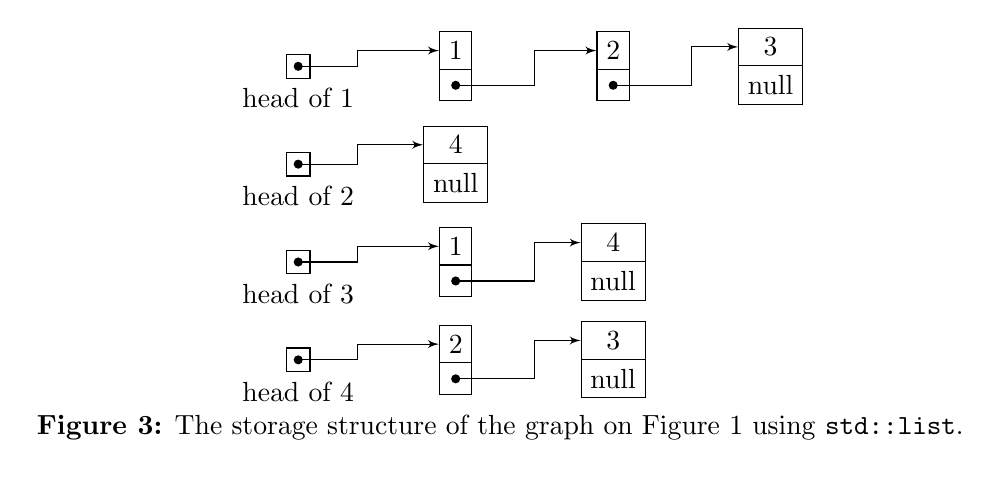
\begin{tikzpicture}[node distance=2cm, auto]

    \node[head, label=below:head of 1] (head1) {};
    \node[data, right of=head1]    (A1) {1};
    \node[data, right of=A1]       (B1) {2};
    \node[data, right of=B1]       (C1) {3 \nodepart{second} null};

    \draw[fill] (head1.center)   circle (0.05);

    \path[ptr]  (head1.center) --++(right:7.5mm)  |- (A1.text west);
    \draw[fill] ($(A1.south)!0.5!(A1.text split)$) circle (0.05);
    \draw[ptr]  ($(A1.south)!0.5!(A1.text split)$) --++(right:10mm) |- (B1.text west);
    \draw[fill] ($(B1.south)!0.5!(B1.text split)$) circle (0.05);
    \draw[ptr]  ($(B1.south)!0.5!(B1.text split)$) --++(right:10mm) |- (C1.text west);
    
    
    \node[head, label=below:head of 2, below of=head1, yshift=5em] (head2) {};
    \node[data, right of=head2]    (A2) {4 \nodepart{second} null};    
    \draw[fill] (head2.center)   circle (0.05);
    \path[ptr]  (head2.center) --++(right:7.5mm)  |- (A2.text west);

	
	\node[head, label=below:head of 3, below of=head2, yshift=5em] (head3) {};
    \node[data, right of=head3]    (A3) {1};
    \node[data, right of=A3]       (C3) {4 \nodepart{second} null};

    \draw[fill] (head3.center)   circle (0.05);

    \path[ptr]  (head3.center) --++(right:7.5mm)  |- (A3.text west);
    \draw[fill] ($(A3.south)!0.5!(A3.text split)$) circle (0.05);
    \draw[ptr]  ($(A3.south)!0.5!(A3.text split)$) --++(right:10mm) |- (C3.text west);
    
    \node[head, label=below:head of 4, below of=head3, yshift=5em] (head4) {};
    \node[data, right of=head4]    (A4) {2};
    \node[data, right of=A4]       (C4) {3 \nodepart{second} null};

    \draw[fill] (head4.center)   circle (0.05);

    \path[ptr]  (head4.center) --++(right:7.5mm)  |- (A4.text west);
    \draw[fill] ($(A4.south)!0.5!(A4.text split)$) circle (0.05);
    \draw[ptr]  ($(A4.south)!0.5!(A4.text split)$) --++(right:10mm) |- (C4.text west);
	\node[xshift=5.3em, yshift=-2em, xshift=2em] (title) 
    at (head4.south)
    {\textbf{Figure 3:} The storage structure of the graph on Figure 1 using \texttt{std::list}.};

\end{tikzpicture}
\end{center}

As shown from Figure 3, \texttt{std::list} doesn't show any cache friendly structure. Thus, usage of it only gives us better update latency.

\subsection{Ajdacency List with \texttt{std::vector}}
Second approach of Adjacency List uses \texttt{std::vector} structure to keep outgoing edges for each node. \texttt{std::vector} also uses an array structure to keep the elements, however whenever it hits the capacity, it creates new doubled size array and copies the contents of the old one including the newly added element, then removes the old one. It may seem to be like a big overhead, but in reality it only does \texttt{3*n} additional operations for \texttt{n} inserts into it. \\

\tikzset{
mymat/.style={
  matrix of math nodes,
  text height=2.5ex,
  text depth=0.75ex,
  text width=3.25ex,
  align=center,
  column sep=-\pgflinewidth
  },
mymats/.style={
  mymat,
  nodes={draw,fill=#1}
  }  
}



\begin{center}

\begin{tikzpicture}[>=latex]
\matrix[mymat,anchor=west,row 2/.style={nodes=draw}]
at (1,1) 
(mat1)
{
 &  &  & \\
1 & 2 & 3 & ?\\
};
\node[] at (0.15,0.93)
  (cella) {\texttt{edges[1]}};

\matrix[mymat,anchor=west,row 2/.style={nodes=draw}, below of=mat1]
at (1.5,1) 
(mat2)
{
 \\
4 \\
};
\node[] at (0.15,0)
  (cellb) {\texttt{edges[2]}};

\matrix[mymat,anchor=west,row 2/.style={nodes=draw}, below of=mat2]
at (1.88,0) 
(mat3)
{
 &   \\
1 & 4 \\
};
\node[] at (0.15,-1)
  (cellc) {\texttt{edges[3]}};

\matrix[mymat,anchor=west,row 2/.style={nodes=draw}, , below of=mat3]
at (1.88,-1) 
(mat4)
{
 &  \\
2 & 3 \\
};
\node[] at (0.15,-2)
  (celld) {\texttt{edges[4]}};



\node[xshift=5.3em, yshift=-1.3em] (title) 
    at (celld.south)
    {\textbf{Figure 4:} The storage structure of the graph on Figure 1 using \texttt{std::vector}.};

\end{tikzpicture}
\end{center}

As it is shown in Figure 4, \texttt{std::vector} implementation also has a cache-fiendly structure.

\section{Evaluation}
All three approches are tested on different datasets which are generated randomly. The number of users differs from 10,000 to 10,000,000. To make it as a real social network, the number of neighbors just differs from 50 to 200. In the following subsections, I discuss in which scenario CSR gives better performance in terms of latency and memory consumption. My test machine is a single socket server computer equipped with Intel(R) Core(TM) i7-3930K CPU 6-core @ 3.20GHz and 64 GB of main memory. This server has 12 hardware cores (with hyperthreading enabled).
\subsection{Experimental platform}

\subsection{Algorithm comparisons}

\subsection{Complex Scenario}

\subsection{Memory consumption}

\subsection{Cache friendliness}

\section{Conclusion}
As it is shown from the results, CSR is not that superior to other two approaches. But considering the fact that social networks are growing so fast nowadays, a slight better approach significantly matters. While most analysis still focuses on static graphs, in the future there will be huge demand on temporal graphs. As CSR itself is not update-friendly, more investigation should be done on the variants of CSR. The CSR library, together with two Adjacency List implementation and generation of graphs, is available online at \texttt{https://github.com/mehemmedv/DB\_Imp\_Seminar}\\

\begin{thebibliography}{}
\bibitem{fb}
Ching, A., Edunov, S., Kabiljo, M., Logothetis, D., \and Muthukrishnan, S. (2015). One trillion edges: Graph processing at facebook-scale. Proceedings of the VLDB Endowment, 8(12), 1804-1815

\end{thebibliography}

\end{document}